\documentclass[14pt,aspectratio=169]{beamer}
\usetheme[version=2019]{iiasa}

\usepackage{ifthen}
\ifthenelse{\equal{\detokenize{notes}}{\jobname}}{%
\setbeameroption{show only notes}%
}{
%
}

% With 14pt
\setbeamerfont{title}{size=\Large}
\setbeamerfont{frametitle}{size=\Large}
\setbeamerfont{section title}{size=\Large}


\usepackage[
  maxnames = 1,
  style = authoryear,
  giveninits,
  terseinits,
  maxcitenames = 3,
  ]{biblatex}
\addbibresource{all.bib}
% Small font in bibliography
\renewcommand*\bibfont{\small}
\addbibresource{all.bib}

\usepackage{minted}
\usepackage{pdfpages}

\usepackage{tikz}
\usetikzlibrary{calc}

\title{Interoperable, reusable data for cross-domain, model-based transport research}
\institute{Energy, Climate, and Environment (ECE) program;
  International Institute for Applied Systems Analysis (IIASA)}

\date{\texorpdfstring{27 March 2022 workshop on “Modelling transport demand in different geographical contexts: assumptions, data, and inclusion of material modelling”, Paris, FR}%
  {2022-03-27}}

\author{\texorpdfstring{Dr. Paul Natsuo Kishimoto \scriptsize\newline
  \href{mailto:paul.kishimoto@iiasa.ac.at}%
       {\ttfamily <paul.kishimoto@iiasa.ac.at>}}%
  {Dr. Paul Natsuo Kishimoto <paul.kishimoto@iiasa.ac.at>}}

\begin{document}

\maketitle

\begin{frame}
\frametitle{Outline}

\tableofcontents

\end{frame}

\begin{frame}
\frametitle{My background}
A modeler:
\begin{itemize}
  \item MIT \structure{EPPA} general-equilibrium (CGE) model family \& linked tools for air quality; health impacts.
  \item Econometrics of household expenditure on transport.
  \item IIASA \structure{MESSAGEix-GLOBIOM} integrated assessment model (IAM) family \& framework.
  \item Fly-on-the-wall for much else.
\end{itemize}

\medskip
\pause
A data user:
\begin{itemize}
  \item Merging data (incl. focused transport models' outputs) to parametrize global, long-term transport/energy/emissions.
  \item IAM \& other model outputs for IPCC AR6 WGIII.
\end{itemize}

\end{frame}

\section{Model-based research and assessment}

\begin{frame}[allowframebreaks]
\frametitle{Model-based research \& assessment}

\begin{columns}
\column{0.65\textwidth}
\includegraphics[height=0.8\textheight]{de-weck-roos-magee-f3.1.png}

\column{0.25\textwidth}
(Transport) systems can be viewed at various levels of abstraction, from various theoretical vantage points.

\medskip

{\small \href{https://mitpress.mit.edu/books/engineering-systems}{de Weck, Roos, Magee (2011) fig. 3.1, p.47}}
\end{columns}

\begin{columns}
\column{0.40\textwidth}
\includegraphics[height=0.8\textheight]{de-weck-roos-magee-f5.2.png}

\column{0.50\textwidth}
Within systems-of-systems, subsystems of the whole have \structure{boundaries}; both internal and boundary-crossing relationships.

\medskip
\structure{Systems phenomena} = things happening within/across 1+ subsystems.

\medskip
{\small \href{https://mitpress.mit.edu/books/engineering-systems}{de Weck, Roos, Magee (2011) fig. 5.2, p.101}}
\end{columns}

\end{frame}

\begin{frame}
\frametitle{Implications}

Research on complex, socio-technical systems always\footnote{for all but the most trivial sub-systems.} implicates \structure{multiple domains}, i.e. is necessarily multi- / inter- / trans-disciplinary.

\bigskip
\pause
\structure{Boundary choices} for \emph{models} usually mirror the extent of concepts and theory in 1+ domain(s); out-of-bounds (exogenous) phenomena can be highly abstracted.

\bigskip
\pause
Domains have their own respective theory, metrology, etc.—all co-evolved.
\pause → Their data thus \emph{look} different and \emph{are talked about} differently, even when they pertain to the same underlying phenomena.

\end{frame}

\section{Challenges in current practice \& their consequences}

\subsection{Data → needs mismatch}

\begin{frame}
\frametitle{1: Data → needs mismatch}

Available data do not match inputs required by methods chosen for modeling and assessment.

\bigskip
\structure{Reponses}
\pause
\begin{itemize}
  \item Make (lots of) assumptions.
    \begin{itemize}
      \item Small vs. large \& “load-bearing”.
      \item Empirically-grounded (analogues, etc.) vs. not (modelers' own intuition/experience/biases).
    \end{itemize}
  \item Construct required data from other data.
    \begin{itemize}
      \item [→] large body of secondary method for this construction.
    \end{itemize}
  \item Measure directly (usually too expensive).
\end{itemize}

\end{frame}

\subsection{Model outputs unclear}

\begin{frame}<1>[label=model-outputs-unclear]
\frametitle{2. Model outputs unclear}

Nature of model outputs is unclear to potential users.
\pause
\begin{itemize}
  \item Distinction between (1) and (2); (3) and (4) is obfuscated.
  \item Buried in supplemental information, in code (if available), or not mentioned at all.
\end{itemize}

\bigskip
\pause
\structure{Responses}
\begin{itemize}
  \item Guess at methods, possibly incorrectly.
  \item Reimplement, at great cost.
  \item Misuse model output data as if they reflect phenomena that are not endogenized.
\end{itemize}

\end{frame}

\begin{frame}
\frametitle{What exactly is “the model”?}

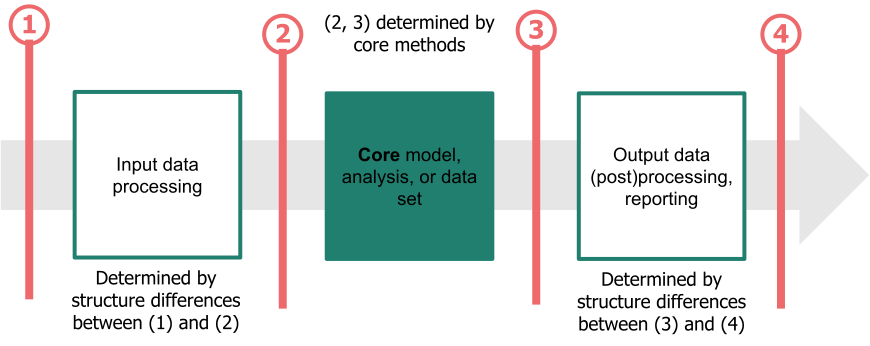
\includegraphics[width=\columnwidth]{data-stages}

\end{frame}

\againframe<2->{model-outputs-unclear}

\subsection{Unreproducible modeling}

\begin{frame}
\frametitle{3. Unreproducible modeling}

Undocumented manual steps \& assumptions mean modeling/analysis is unreproducible…
\begin{itemize}
  \item …by the same researcher(s) who originally did the work.
  \item …by anyone else.
\end{itemize}

\bigskip
\pause
\structure{Responses}
\begin{itemize}
  \item Invent a new model.
  \item Fall back to simpler, older, poorer methods that \emph{are} documented or reproducible.
  \item Supplicate model owners to transfer practical knowledge through collaboration, consulting.
\end{itemize}

\end{frame}

\subsection{Incentive to complicate, not validate}

\begin{frame}
\frametitle{4. Incentive to complicate}

Social \& systemic incentives to increase sophistication, complexity, etc.
\begin{itemize}
  \item Innocent reasons: it's fun/cool; stakeholders ask for it.
  \item Neutral: high-impact journals select for novelty; career advancement requires publication in these journals.
  \item Malicious: preserve an advantage over perceived ‘competitors’.
\end{itemize}

\bigskip
\pause
\structure{Responses}
\begin{itemize}
  \item Complexity arms race; many incompatible models.
  \item Deprioritize and de-resource validation, data production, \& preparation.
\end{itemize}

\end{frame}

\begin{frame}
\frametitle{Consequences}

(O)FAIR—OFA in practice, I \& R at best notional.

\medskip \pause
Leading-edge methods—developed \& applied in data-‘rich’ contexts—grow increasingly irrelevant for data-‘poor’ contexts.%
\begin{itemize}
  \item Inequity in data availability mirrors \& amplifies broader inequity.
\end{itemize}

\medskip \pause
Barriers to entry, participation, etc. are unjustifiably high.

\medskip \pause
Not enabling broad transitions to sustainability.

\medskip \pause
Not sustainable: crisis of legitimacy for entire disciplines \& their collective output.

\end{frame}

\section{Fixes \& directions}

\subsection{Talk about \emph{data flows}}

\begin{frame}
\frametitle{Talk about \emph{data flows}}

Emphasize \structure{data flows} in to/out of models, as much as or more than model contents.

\begin{columns}
\column{0.45\textwidth}
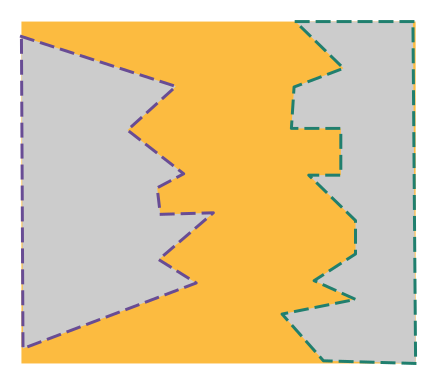
\includegraphics[height=0.7\textheight]{data-gap}

\column{0.45\textwidth}
\pause \small
Many benefits:
\begin{itemize}
  \item Clarify system boundaries.
  \item Clarify endogenized vs. exogenous phenomena.
  \item Allow would-be model users to gauge data prep work.
  \item Allow consumers of output data to use them correctly.
\end{itemize}
\end{columns}

\end{frame}

\subsection{Describe the \emph{structure} of data}

\begin{frame}
\frametitle{Describe the \emph{structure} of data}

…both inputs/outputs.
SDMX standard provides file formats for sharing this information.

\bigskip
Precisely define background concepts and systematized measures.
Then—for \emph{each \& every one}—state clearly:
\begin{itemize}
  \item Units of measure.
  \item \structure{Dimension(s)}: time, space, mode, vehicle type, demographics, …
  \item \structure{Scales} along those dimensions.
    \begin{itemize}
      \item Discrete: lists of codes (labels) and their meanings.
      \item Continuous: scope and resolution.
    \end{itemize}
  \item Other attributes and metadata; or references thereto.
\end{itemize}

\end{frame}

\subsection{Establish \& apply standards}

\begin{frame}
\frametitle{Establish \& apply standards}
\framesubtitle{→ Transport Data Commons (TDC) — §3 later today}

Establish community standards; apply; \structure{disseminate} broadly; \structure{train} data providers; \structure{iterate}.

\bigskip
\pause
Learn from domains that have already undergone revolutions:
\begin{itemize}
  \item Climate science/Earth system modeling; physical sciences.
  \item Industrial ecology; power systems.
\end{itemize}

\bigskip
\pause
Initial, rudimentary steps:
\begin{itemize}
  \item Official statistics.
  \item IPCC \& Integrated Assessment Modeling Consortium.
  \item Int'l Transport Energy Modeling (iTEM) Open Data.
\end{itemize}

\end{frame}

\begin{frame}
\frametitle{Thank you}

Hopes from this talk:
\begin{itemize}
  \item Vocabulary, concepts, motivation for *-disciplinary discussions about transport models.
  \item Spotter's guide to practices that work \emph{against} interoperable and reusable data.
  \item Think about how to work towards genuinely accessible transport research methods \& suitable data.
\end{itemize}

\end{frame}

\end{document}
